\title{Rendering and Optimization of Gaussian Radiance Fields}

\author{Valerie Dagley, Cameron Durbin, Andrew Rehmann}

\newcommand{\abstractText}{\noindent
In this paper, we present a high level overview of a recent paper, 3D Gaussian Splatting for Real-Time Radiance Field Rendering \cite{kerbl20233d}. We also detail our implementation of a similar renderer, and other steps we took to replicate this paper. While we didn't fully succeed in replicating all steps of the paper, we did create a recognizable image, as well as started some of the important building blocks of the algorithms used in the paper. For example, the GPU parallel prefix sum, which is at least 40 times faster than a simple serial CPU version.
}

%%%%%%%%%%%%%%%%%
% Configuration %
%%%%%%%%%%%%%%%%%

\documentclass[12pt, a4paper, twocolumn]{article}
\usepackage{xurl}
\usepackage[square, comma, numbers, sort]{natbib}
\setcitestyle{numbers, open={[}, close={]}}
\usepackage{abstract}
\renewcommand{\abstractnamefont}{\normalfont\bfseries}
\renewcommand{\abstracttextfont}{\normalfont\small\itshape}
\usepackage{lipsum}
\usepackage{amsmath} 
\usepackage{algorithm, algpseudocode, algorithmicx}
\usepackage{graphicx, tabularx}


\usepackage{titlesec}

\titleformat{\section}
  {\normalfont\fontsize{14}{14}\bfseries}{\thesection}{0.5em}{}

\titleformat{\subsection}
  {\normalfont\fontsize{12}{12}\bfseries}{\thesubsection}{0.5em}{}


%%%%%%%%%%%%%%
% References %
%%%%%%%%%%%%%%

% If changing the name of the bib file, change \bibliography{test} at the bottom
\begin{filecontents}{workscited.bib}
@misc{kerbl20233d,
  title={3D Gaussian Splatting for Real-Time Radiance Field Rendering}, 
  author={Bernhard Kerbl and Georgios Kopanas and Thomas Leimkühler and George Drettakis},
  year={2023},
  eprint={2308.04079},
  archivePrefix={arXiv},
  primaryClass={cs.GR}
}
@misc{barron2022mipnerf,
  title={Mip-NeRF 360: Unbounded Anti-Aliased Neural Radiance Fields}, 
  author={Jonathan T. Barron and Ben Mildenhall and Dor Verbin and Pratul P. Srinivasan and Peter Hedman},
  year={2022},
  eprint={2111.12077},
  archivePrefix={arXiv},
  primaryClass={cs.CV}
}
\end{filecontents}

% Any configuration that should be done before the end of the preamble:
\usepackage{hyperref}
\hypersetup{colorlinks=true, urlcolor=blue, linkcolor=blue, citecolor=blue}

\begin{document}

%%%%%%%%%%%%
% Abstract %
%%%%%%%%%%%%

\onecolumn
\maketitle
\begin{abstract}
    \abstractText
\end{abstract}

\twocolumn

%%%%%%%%%%%
% Article %
%%%%%%%%%%%

\section{Introduction}

The topic of novel view synthesis is a large and ongoing research area. Novel view synthesis (NVS) is the process of taking a set of images of a scene and generating new images from viewpoints not covered by the original data set. We attempted to re-implement a recent NVS approach utilizing 3D Gaussians to create a scene representation capable of real time rendering of novel views. This project was done in two sections--the model training and the Gaussian renderer.

Our approach was based on one by Kerbl et. al. \cite{kerbl20233d}. They propose a unique scene representation using 3D Gaussians (points with a sphere of influence, with a transparent ``fog'' tapering off with distance) to convert a point cloud representation into a differentiable volumetric representation. Their approach begins by generating a point cloud from a set of images using a structure from motion (SfM) algorithm \cite{Ko2016PointCG}. Using this as a basis, they create a set of Gaussians. They then optimize this set by splitting, merging, and adjusting different parameters to minimize the total loss between the rasterized result and the reference dataset. Because a key part of this optimization process is comparing the rasterized result to the references, the rasterizer must be very fast. They propose a tile based parallel CUDA rasterizer that allows realtime rasterization of millions of Gaussians with minimal error. Through the combination of the training model and the rasterizer, their system can create near-photorealistic novel views based on relatively small sets of images.

\section{Methodology}

Our project was implemented entirely in C++ utilizing CUDA and OpenMP for parallel programming. We initially split our project into two separate sections, hoping to keep them independent and only reliant on each other in minimal ways. 

\subsection{Training Model}

Building a 3D scene from images requires a dense, iterative procedure to process all the details from a collection of images. The procedure consists of building the training set, mapping 3D gaussian distribution to their rightful position and shape in the scene, and measuring the similarity of the newly generate scene against the reference scene. The training procedure will be broken down into 3 sections: initialization, gradient descent, and Termination.

\subsubsection{Initialization}

Training data is represented as a set of 2D images captured from different angles and lighting conditions. Each image is paired with a depth map that describes the distance from the camera to each point in the scene. The training process begins with loading the information about each image and their depth map in arrays. Camera lens have specific distortions of the view they capture so a computational correction must be applied to each image. Following the correction of each camera's view of the image, we compute the Neural Radiance Field for each image. This computation consists of taking the transpose and inverse of the camera's 4x4 information matrix which was performed with CUDA in this project. Once the training set is complete, it's ready to be processed by the optimizer, gradient descent.

\subsubsection{Gradient Descent}

Gradient descent is an optimization algorithm that aims to reduce a loss function to zero. In this project, our loss-function is the following:

\begin{equation}
    \mathcal{L} = (1-\lambda)\mathcal{L}_1 + \lambda \mathcal{L}_{D-SSIM}
\end{equation}

where 

\begin{equation}
    \mathcal{L}_1 = \sum_{i=1}^{n} |y_i - f(x_i)|
\end{equation}

and $\mathcal{L}_{D-SSIM}$ is the Structural Similarity Index Measure of the image. This measurement consists of differences between brightness, contract, and other image qualities. It is widely recognized in the image processing.

The loss function represents how different the generated image is from the reference image. We can take advantage of this loss function by computing the derivative of the loss function with respect to each gaussian point and adjust the points a step closer to the reference image. By taking the derivative of a gaussian point, we are taking the derivative of the gaussian point with respect to the distribution's position and standard deviation in each axis (x, y, z) as well as the transparency. These are the values that we adjust to reduce the error of our equation. At the end of each epoch, we begin a procedure for removing gaussian points and splitting gaussian points. When two gaussian points are overlapping or not adding any detail to the image, we remove a guassian. And when a gaussian can't fit into a specific shape, the guassian splits and allows for a new gaussian to fit into the missing space. The algorithm is as follows:

\begin{algorithm}
\caption{Gradient Descent}
\hspace*{\algorithmicindent} \textbf{Input:} $\Theta, \hat{I}, E_p, \eta$\\
\hspace*{\algorithmicindent} \textbf{Output:} $\hat{\Theta}$
\begin{algorithmic}[1]

\Procedure{GradDescent}{}
    \For{$i = 1$ to $E_p$}
        \State $I \leftarrow \text{rasterize}(\Theta)$
        \State $g \leftarrow \frac{1}{m} \sum_{j=1}^{m} \nabla \text{Loss}_j(I, \hat{I})$
        \State $\Theta \leftarrow \Theta - \eta g$
        \State $\Theta \leftarrow \text{Rmv/Splt}(\Theta)$
    \EndFor
    \State \Return $\hat{\Theta}$
\EndProcedure
\end{algorithmic}
\end{algorithm}

\subsubsection{Termination}

A threshold close to $0$ should be specified in order to capture the model at a specific accuracy. Once the $Loss$ of the newly created image and the reference image crosses the threshold, the model should be exported for use.

\subsection{Renderer}

The renderer is an essential part of this method. Because it is used as a key step in the training algorithm, it must be extremely fast to allow for efficient training. 

A trained model will typically consist of between 1 and 10 million unique Gaussians--each with their own unique scale, rotation, and ``mean'' (the center point of the Gaussian distribution). In order to render them in any reasonable amount of time, a good renderer should have a way to cull any of the Gaussians outside of the view of the camera (to prevent them from being calculated unnecessarily). On top of this, it needs to be able to sort the Gaussians by their distance from the camera in order to properly blend the partially transparent parts of the distribution. The method proposed in the paper combined both of these (as well as a rasterization speedup) into a solution utilizing screen-space tiles. 

\subsubsection{Rasterizer}

Before getting to the optimizations of the renderer, we had to implement a rasterization method for the transformed Gaussians. As mentioned earlier, each Gaussian is represented using a position (the ``mean'' of the distribution), a 3D rotation, and a non-uniform scale. These 3 values for each Gaussian represent a unique affine (linearity-preserving) transformation applied to the ``unit'' Gaussian (the 3D Gaussian distribution with mean at the origin and uniform standard deviation of 1 unit in all directions). The renderer also associates an RGB color and an opacity value for each Gaussian. 

It is relatively simple to render the unit Gaussian distribution--simply fire a ray out of the camera origin for each pixel, then determine how much the Gaussian distribution ``accumulates'' along that ray. In our implementation, this is done via a ``ray marching'' solution- instead of deriving equations for how any arbitrary ray interacts with the unit Gaussian, simply choose a set of arbitrary points along that ray and measure the influence of the Gaussian at each of those points. The influence of the unit Gaussian on a single point is trivial- because a 3D Gaussian is radially symmetric you can calculate a 1D Gaussian function on the distance of the point from the origin. In the rendering, we will use the influence of a Gaussian on a ray as the ``alpha'' (transparency) modifier for the final pixel color.

To render any arbitrarily (affine) transformed Gaussian, we can exploit the fact that all affine transformations have a simple inverse transformation. we begin by generating a unique ray for each pixel on the screen (in practice, we only generate rays for pixels that will actually be influenced by the Gaussian in a meaningful way). These rays are initially generated in ``world space''--originating from the camera position and pointing in the direction the camera is facing. Then, for each Gaussian $G_i$, we find the values $r_i, t_i, s_i$ representing the transformations (rotation, translation, scale) applied to transform the unit Gaussian into $G_i$. We can then apply the inverses of all three transformations to our generated rays for each pixel to get a ``model space'' ray. Geometrically, we have applied these transformations to the entirety of the ``world space'' which means that the Gaussian $G_i$ has now been transformed \textit{back} into the unit Gaussian. Now that we have our ``model space'' ray, we can simply apply the algorithm previously described to find the influence of the Gaussian $G_i$ along the specific ray. As mentioned before, the influence of a Gaussian on the ray represents the alpha modifier for the final pixel color. In order to calculate the pixel color from the Gaussian, we take the base opacity of the Gaussian $G_i$ and multiply it by the alpha modifier. This modified opacity value can then be used with the base color of the Gaussian to draw to the screen.

In order to speed up this ray marching calculation (which can be very slow if too many points are chosen or inaccurate if poor points are chosen), we also use another approximation. The majority of the influence of the unit Gaussian on any specific ray will happen inside the unit sphere--so instead of calculating the influence on the entire ray, we can intersect that ray with the unit sphere and calculate the influence on the inside of the unit sphere only. This approximation works extremely well--so much so that as little as 3 points can be sampled for a quality approximation of the Gaussian influence. It also allows for early exits in the case that a ray does not intersect with the unit sphere, but we did not use this fact in order to minimize thread divergence on the GPU (however we do not consider the influence of the Gaussian on a ray that does not intersect the unit sphere).

Once we are able to render a single arbitrary Gaussian distribution, very little is left to extend the renderer to be able to draw many together. As mentioned earlier, each pixel will have a calculated opacity and base color for all of the Gaussians that influence that pixel. These must be alpha-blended in depth order to properly find the final pixel color to draw to the screen. We use the a multiplicative alpha blending function to handle this.  

In theory, this set of calculations is well within the ability of modern GPUs. However, with multiple million relatively small Gaussians, this gets extremely computationally expensive. One of the largest inefficiencies in a naive implementation of this method is the fact that many of the Gaussians have little to no influence on most of the pixels on the screen. On top of this, a naive implementation of this method would be unable to distinguish Gaussians that appear on screen from those that do not. The paper proposing this method used an optimization that solved both of these issues at once. Instead of attempting to render every Gaussian to every possible pixel, split the screen up into small tiles that then only render the Gaussians that contribute to the pixels in each tile.

\subsubsection{Tile Rendering}

The concept behind a tile-based renderer is relatively simple. Instead of considering how to render the entirety of the screen at once, subdivide the screen into many small tiles that can be rendered separately. This solves quite a few issues in computer graphics in general, allowing large serial operations to be done in smaller parallel batches. In our specific case, it solves three main issues: drawing Gaussians outside of the camera view, doing calculations on Gaussians that will never affect a specific pixel, and the complexity of sorting large numbers of Gaussians. However, in order to use a tile based renderer, we need to add a few extra steps to the rendering algorithm. These will all be applied on the set of all Gaussians before they are considered for rendering (minimal changes are needed to the rasterization algorithm).

First, we need to know what Gaussians are visible from a specific tile. The section of world space visible from the camera is described by the \textit{view frustum}, or more simply, a \textit{view pyramid} (the difference between a frustum and a pyramid is relatively unimportant for the algorithm). The view pyramid consists of 4 planes that represent the edges of the screen. In order to determine if a Gaussian is inside the view pyramid, we check if it is inside the section of space between the 4 planes. This is a relatively simple check for the unit Gaussian but very complex for an arbitrary Gaussian, so we will use the same method as before (applying the inverse transformations for each Gaussian and calculating in that ``model space''). In order to determine the section of world space visible from a specific tile, we will determine the planes that represent the edges of that tile. This is done by subdividing the view pyramid in the exact same way we subdivide the screen space--being careful to insure that `partial tiles'' (which may not be fully on screen) are handled correctly. Once we can determine the planes that represent the edges of each tile, we can perform the same culling check as with a larger view pyramid. (note: the view pyramid for most of the tiles will be skewed from a simple pyramid, but culling using the planes of each face of the pyramid still works exactly the same). 

Now that we know how to determine if a Gaussian is inside the view pyramid, we can perform this check on all of the Gaussians in the scene before we begin rendering. This will also remove any Gaussians that are not visible from the camera. If a Gaussian is visible from a specific tile, we add it to a bin corresponding to that tile. In our implementation, each bin is a constant size--this simplifies the implementation but causes some issues with rendering dense sections of the screen. 

Once all of the Gaussians are placed into their proper bins they can be rasterized using the previously described algorithm, except that instead of calculating the contribution of every single Gaussian, we only calculate the contribution of the Gaussians of the tile a pixel resides in. This limits the number of calculations required for each pixel, which allows for an extremely large speedup over the naive implementation.

\subsubsection{Depth Sorting}

As mentioned earlier, Gaussians have to be alpha blended in depth-order. Our implementation handles this after the tile binning step for simplicity. We apply a simple GPU even-odd sort to the Gaussians in each tile to sort them back to front. This sort is done by assigning each block to a specific tile. We then calculate the distance from the camera for all of the Gaussians in that tile and place those values in the GPU block-shared memory. We can then apply the sorting algorithm to the shared memory set of keys, moving the associated Gaussians inside the bins alongside them. However, because this utilizes a 32 bit floating point key for each Gaussian in a tile bin, it limits the maximum bin size to 12,288.

Once the Gaussians are sorted, we can render them in that order using the painters algorithm to get the final pixel colors for each pixel. 

The paper implements depth sorting and binning in a slightly different manner. Rather than separating these two processes, it actually combines them into one. For every Gaussian, it calculates an associated number of tiles that it covers. Then, it can use a prefix sum to know both an amount of memory to allocate, as well as a location to place a certain number of duplicates of each Gaussian. Each Gaussian is duplicated according to the number of tiles that it occupies, and can be placed into this new array in parallel, as each has its own independent area in the array.

These new, duplicated Gaussians then have a key associated with each of them, where the highest order bits of the key are based on the tile they cover and the lowest order bits of the key are assigned to be the viewspace depth of the Gaussian. Then, the paper performs a radix sort on the Gaussians based on these keys. In this way, the Gaussians are now grouped based first on tile ID, and then on their depth from the camera. Each thread block spawned for the rendering can then take a pointer to somewhere in this new sorted array as the start of the array for its tile. This allows for variable size arrays for each thread block, which gives the possibility of more detail for the detailed sections, but no over-allocation in the less detailed areas.

It was for this reason that we also began to implement a GPU based parallel prefix sum, as this algorithm is clearly heavily used. Not only for checking the amount of memory to allocate and where to duplicate the Gaussians, but radix sort can also be built off of a prefix sum. If you have a set of keys that are to be sorted based on unsigned binary size, you can mask to get the least significant bit, and prefix sum by treating those as ones. Then, with a subtraction or two,
you can use this prefix sum to tell you where to put this object you're sorting. If you repeat this, moving up to the next most significant bit every step, you will have sorted your elements. 

A GPU parallel prefix sum is nearly the same as the work-efficient CPU parallel prefix sum, however there are still some differences. It would be inefficient to assign a single thread block to the entirety of your data, however thread blocks can't really communicate with each other without finishing the kernel. It's for this reason that a GPU parallel prefix sum actually calls several kernels. First, each thread block performs a prefix sum over its section of the array, and then if it is any section of the array
other than the last, it gathers the final value into an auxiliary array. This auxiliary array is now also
scanned, in order to get an amount to add to each corresponding section. Then, each value in this auxiliary array is applied back to a section of the larger array, which gives each section its proper value.

\section{Results}

\subsection{Training Model}

The training for the model saw efficient parallelization in the initialization portion of the training. Applying parallelization techniques to compute the transpose and inverse of each camera's depth matrix saw a 1.36x and 1.23x speedup respectively. I believe that this speedup isn't as fast as we'd like it to be because of the data transfer latency from the memory to the GPU. Unfortunately we weren't able to compute the gaussian point gradients in parallel due to time restrictions.

\subsection{Renderer}

The renderer turned out to be much more difficult than expected. Our understanding of the algorithm was relatively well developed when we began implementation, but the actual code behind the renderer turned out to be much more complicated. Initially, we precomputed the affine transformation (and their inverses) before the renderer even began. However, this turned out to be a poor idea as it abstracted away some of the bugs that became obvious if you treated each transformation individually. These transformation bugs were some of the most prevalent throughout the development of the renderer, causing most of the testing renders to be completely unintelligible. 

In order to be able to program the renderer in separate from the training code, we used the provided pre-trained models made available by the authors of the original paper. These were provided in the .PLY file format and very minimally documented, so most of the file parsing was done by assumption (and a lot of interpreting their code). This also caused numerous problems, as small errors in the file parsing cause the Gaussian data to be fully corrupted. The largest error we had was with the rotations, which are stored as 4 floats representing the components of a Quaternion. In the file, these are stored in WXYZ order. If interpreted in any other order, the rotation data is completely corrupted. This is not documented anywhere. On top of this, the .PLY data stores the opacity in a way that needs to be activated by a sigmoid function and the scale in a logarithmic format. 

Once we had sorted out all of the issues with getting and applying the transformations to each Gaussian properly, we had to figure out how to calculate the colors. The colors in the renderer are calculated via a Spherical Harmonic lighting calculation, which we deemed to be too complex early on. We simply used the first 3 coefficients of this, which represent the ambient terms. However, these also have to be adjusted to get the final colors for the screen.

After getting most of the bugs and small issues sorted, we ended up with a relatively fast renderer that is able to \textit{almost} draw correct images based on pre-trained data. We ended up running into an issue where the scale of the Gaussians needs to be modified based on a value calculated from the training images, which we were unable to replicate. However, it is still \textit{nearly} possible to see the target image in our renders.

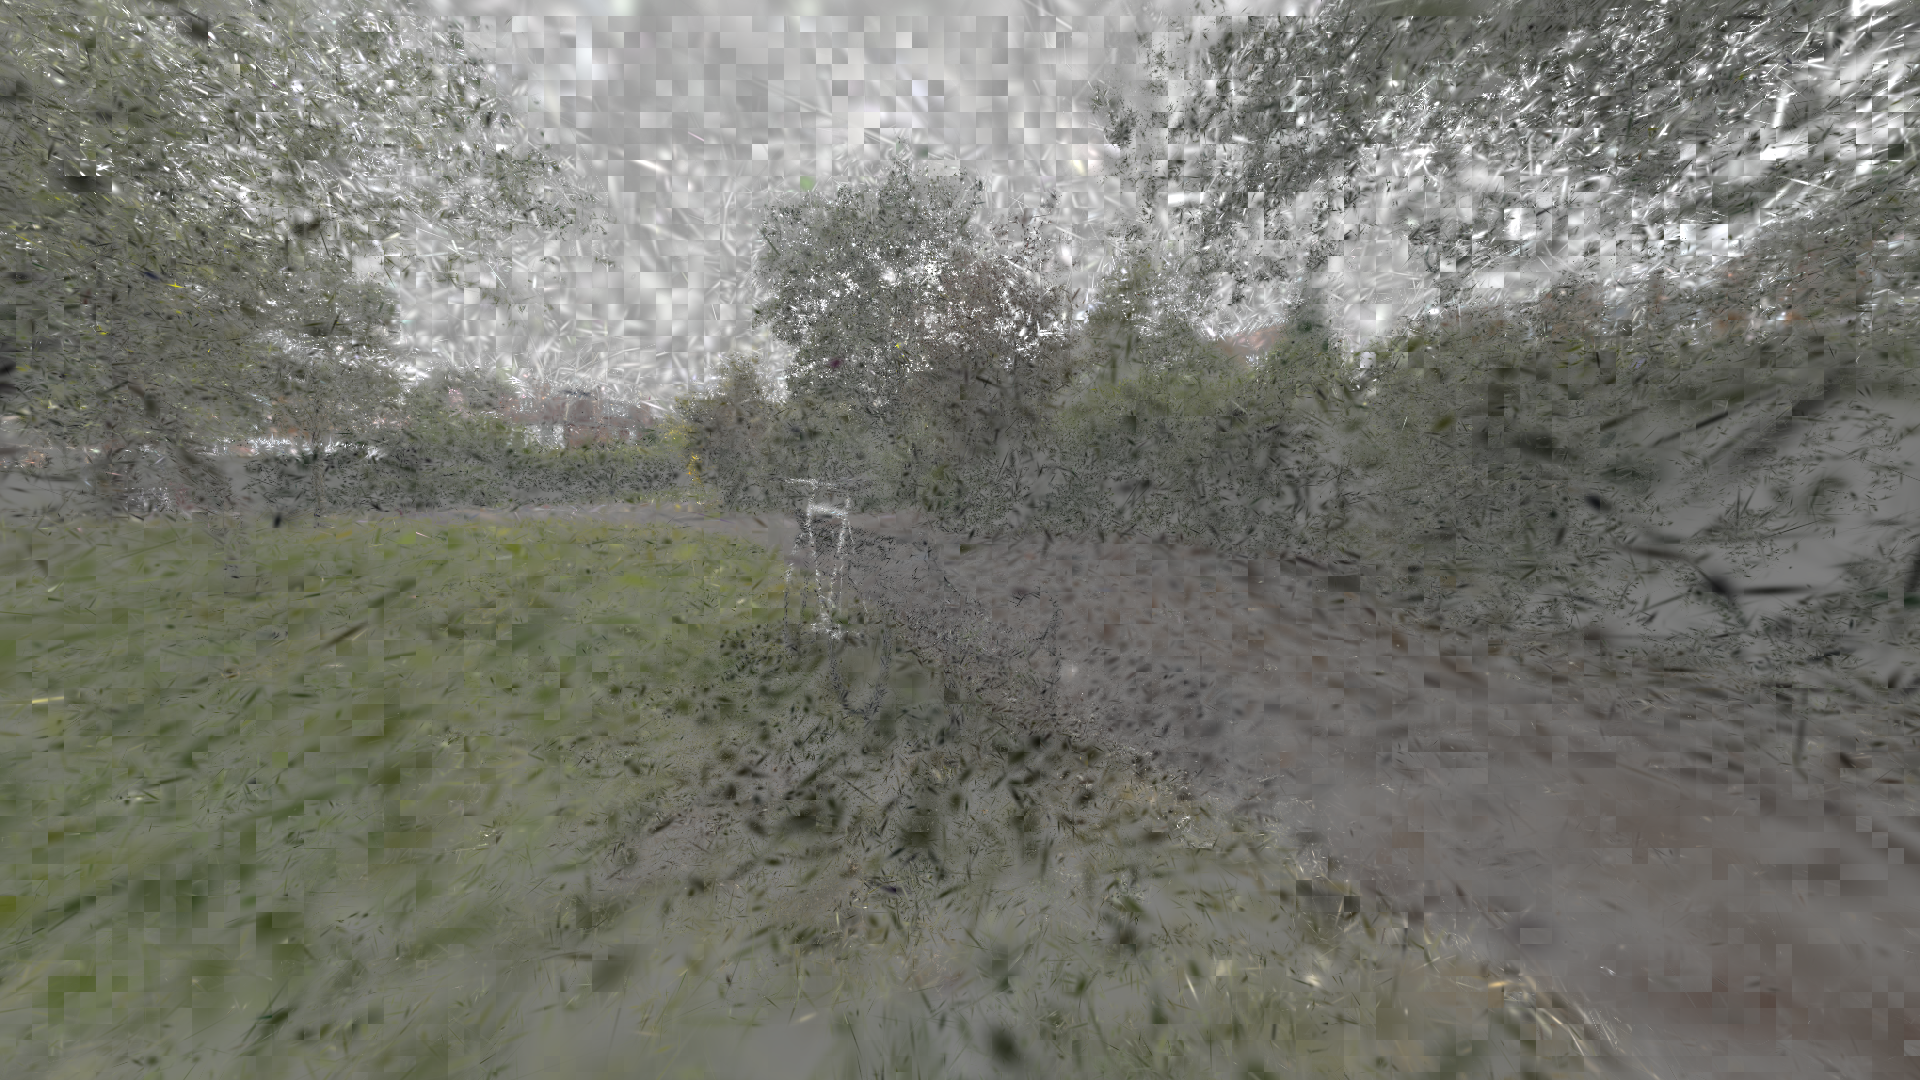
\includegraphics[width=0.425\textwidth]{test.png}

\begin{center}
\begin{tabular}{ | c | c | }
\hline
Operation & Time (ms) \\
\hline
Tile binning & 6282.0166ms \\
\hline
Tile sorting & 235.6890ms \\
\hline
Rasterization & 862.6944ms \\
\hline
Total time & 7380.3100ms \\
\hline
\end{tabular}
\end{center}

The time to render this image on a 3070 Laptop GPU was roughly 8 seconds. This is nowhere near the 150fps that the original paper achieved, but very solid for a first implementation without having much experience in CUDA. This image was rendered at 1920x1080 pixels and the pre-trained model contained 6.1 million unique Gaussians. It used a 16x16 tile size with a maximum of 12,288 Gaussians per bin.

\subsubsection{Prefix Sum}
The GPU parallel prefix sum ran, unsurprisingly, much faster than a serial prefix sum on the CPU. It should be noted that these times are only for the prefix sum algorithm itself, not the time taken to copy the data from the CPU to the GPU. This is because the use of the prefix sum algorithm in the paper would have been on memory already in the GPU, so there wouldn't be a need to copy the data to the GPU.
All timings are based on 20 runs.

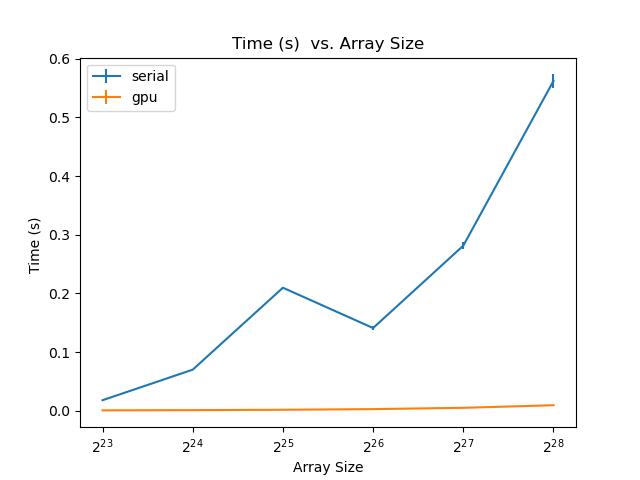
\includegraphics[width = 0.425\textwidth]{time vs arr_size-serial-gpu.png}

It's a bit hard to actually see the speed of the GPU parallel prefix sum, so instead, here is a graph of the speedup as compared to the serial CPU algorithm:

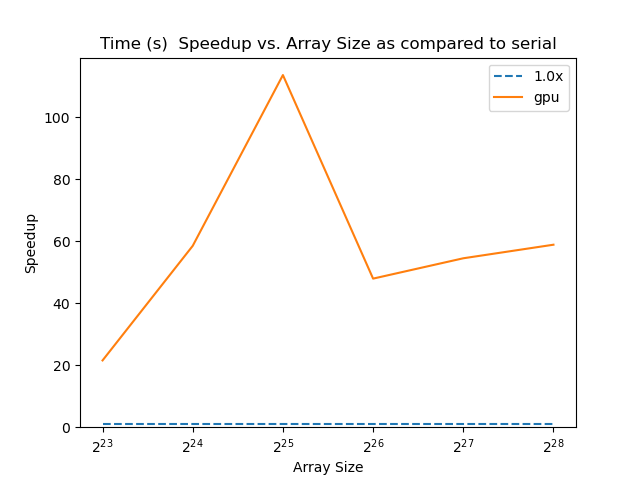
\includegraphics[width = 0.425\textwidth]{Speeduptime vs arr_size-serial-gpu.png}

The GPU algorithm peaks at 100x faster than the serial CPU algorithm. Now, this is cherry-picking data in a way, as this doesn't include the hefty time cost of moving data to the GPU. However, as mentioned above, this is not an unrealistic scenario in the context of a renderer already having this data for use in the GPU.

\section{Conclusion}
In this paper, we detailed the steps required to both train and render a Gaussian model of a scene. The model would have been trained using gradient descent in order to minimize the loss from the reference images. Unfortunately, a lot of time was spent trying to understand the method that the paper used to implement this gradient descent, as their back-end was in PyTorch. After abandoning this to some degree, little time was left to get at least some parallel programming. The renderer we created was not nearly as efficient as the one outlined in the paper, however this is expected, as it was the first time working in CUDA for most of us on this project. Despite that, it produces a recognizable image of the scene, which is a decent achievement considering the unusual nature of the objects being rendered. The prefix sum algorithm was very efficient, but we did not have time to build much off of it. If we had focused our efforts on more concrete aspects of the paper that we knew we could implement, we would have perhaps had more completed segments to show. As-is, there is still a large amount of GPU code which is either infeasible to execute in a serial manner, or demonstrably much faster in a parallel context.


\subsection{Future Research Directions}
As we chose a bit of an ambitious project, we weren't able to get nearly the polished product we were looking to. Thus, there are many possible opportunities for research directions. One would be to reimplement the rasterizer as outlined by the paper, and compare our more volumetric 3D method to their splatting. A step along that path would be to implement a radix sort based on the existing prefix sum algorithm that we have. In addition, the prefix sum was made to allow a variable amount of work per thread, however that complicated the indexing enough that we weren't able to get it working as a general case. Modifying the code to allow for a thread block to process more elements than the number of threads it has may give a slight speedup, with better work distribution. GPU code, even more than CPU code can have optimizations that are very hardware specific, so it would be a good continuation to allow for easier parameter tuning in this code.



%%%%%%%%%%%%%%
% References %
%%%%%%%%%%%%%%

\nocite{*}
\bibliographystyle{plainnat}
\bibliography{workscited.bib}

\end{document}
